\chapter{Computation and Applications of an Optimal Transport}
The approximation of an optimal transport is a computationally expensive problem.  In this chapter we present the discrete formulation of the Kantorovich's problem. We can see that the discrete Kantorovich's problem is a subcase of a general linear program.
%We can attack this problem by the approaches of \textbf{First  Discretize then Optimize} or \textbf{First Optimize then Discretize}
\section{Discrete Formulation and Linear Programming.}
We denote by $\one_n=\parentheses{1,1,\dots,1}^\top\in \Real^n$ the vector composed of $n$ $1$'s. The vector composed of $n$ $0$'s is denoted by $\zeros_n=\parentheses{0,0,\dots, 0}^\top\in\Real^n$. We call a simplex $\Sigma_n$ the convex set of vectors $\pmb{p}=\parentheses{p_1, \dots, p_n}^\top\in \Real^n$ such that, 
\begin{equation}
	\Sigma_n=\braces{\mathbf{p} \in \Real^n: \ \sum_{i=1}^{n}{p_i}=1\ \mand\ \mathbf{p}\geq 0 }.
\end{equation}
Let $X=\braces{x_1, x_2, \dots, x_n}$ be a finite set of $n$ elements. Let $\mu$ a probability measure defined over $X$. Since $X$ is a finite set, we can express the probability measure $\mu$ as follows,
\begin{equation}
	\mu=\sum_{i=1}^{n} a_i \delta_{x_i},
\end{equation}
where $\mathbf{a}=\parentheses{a_1, a_2, \dots, a_n}^\top \in \Sigma_n$. In this section we represent the Kronocker's delta $\delta_{x_i}: X\to \braces{0,1}$ defined over a finite set $X$ by the equation,
\begin{equation*}
\forall x_i\in X\quad	\delta_{x_i}(x)=\begin{cases}
	1 & x=x_i \\
	0 & x\neq x_i
	\end{cases}.
\end{equation*}  
Hence, we have that $\mu(x_i)=a_i$ for all $x_i\in X$. Using the same notation, let $Y=\braces{y_1, y_2, \dots, y_m}$ be a finite set of $m$ elements. Let $\nu$ be a probability measure defined over $Y$ defined by,
\begin{equation}
	\nu=\sum_{i=1}^{m} b_i \delta_{y_i},
\end{equation}
where $\mathbf{b}=\braces{b_1, b_2, \dots, b_m}^\top\in \Sigma_m$,  and $\delta_{y_i}: Y\to\braces{0,1}$ is a Kronecker's delta defined on $Y$. We see that $\mu$ and $\nu$ are identified by a vector $\mathbf{a}\in \Sigma_n$ and $\mathbf{b}\in \Sigma_m$ respectively. 

We can construct a coupling between $\mu$ and $\nu$, using matrix notation. Let $\mathbf{M}^{n\times m}\ni\pmb{\gamma}$ be a matrix of $n\times m$ real entries, i.e. $(\pmb{\gamma})_{i,j}$ with its marginals given by $\mathbf{a}$ and $\mathbf{b}$,
\begin{align}
	 \pmb{\gamma}\, \one_m=\sum_{j=1}^{m}\gamma_{i,j}=a_i\quad \mand \quad \pmb{\gamma}^\top\one_n=\sum_{i=1}^{n}\gamma_{i,j}=b_j \label{eq: matrix prob marginals}
\end{align}
From the equation \ref{eq: matrix prob marginals},  and the fact that $\mathbf{a}\in\Sigma_n$, we can see that the sum of all the entries of $\pmb{\gamma}$ is also $1$,
\begin{equation}
 	\sum_{i=1}^{n}\sum_{j=1}^{m}\gamma_{i,j}=\sum_{i=1}^{n}a_i=\sum_{j=1}^{m}\sum_{i=1}^{n}\gamma_{i,j}=\sum_{j=1}^{m}b_j=1 
 \end{equation}
Therefore we can see $\pmb{\gamma}$ as a joint probability measure over the space $X\times Y$ with marginals given by $\mu$ and $\nu$.

Let $c:X\times Y \rightarrow \Real$ a cost function. The $X$ and $Y$ are finite sets with $n$ and $m$ elements respectively, therefore we can use a matrix $\mathbf{C}\in \mathbf{M}^{n\times m}$ to represent the cost function.
\begin{equation}
	(\mathbf C)_{i,j}=c_{i,j}=c(x_i, y_j).
\end{equation}

We see that the dimensions of $\mathbf{C}$ are equal to the dimensions of $\pmb{\gamma}$. Then given a transportation plan between $\mu$ and $\nu$ the total cost is given by,
\begin{equation}
	\anglesbox{\mathbf{C}, \pmb{\gamma}}=\sum_{\substack{1\leq i \leq n \\ 1\leq j\leq m}}c_{i,j}\gamma_{i,j}=\tr\parentheses{\mathbf{C}^\top\pmb{\gamma}},
\end{equation}
where $\anglesbox{\cdot, \cdot}$ in this setting is the Frobenius inner product \footnote{For matrices with real entries the product is defined as $\anglesbox{A, B}=\tr(A^\top B)$.} of the two matrices.
\subsection{Linear Programming Notation.}
As mentioned before, the discrete formulation is a specific case of linear programming in finite dimensions. Given the discrete analysis presented above the transportation problem is reduced to,
\begin{equation}
	\Theta(\mu, \nu)=\min_{\pmb{\gamma}\in \Pi(\mu, \nu)}{\anglesbox{\mathbf{C}, \pmb{\gamma}}}\label{eq: Optimal Cost Frobenius}
\end{equation}
The vectorization $\mathrm{vec}(\mathbf{R})$ of a matrix $\mathbf{R}\in \mathbf{M}^{n\times m}$ is a linear transformation which converts the matrix into a column vector $\mathbf{m}\in \Real^{mn}$. If $\mathbf{z}\in \mathbf{M}^{1\times n}$ is one row matrix, we see that its vectorization $\mathrm{vec}(\mathbf{z})=\mathbf{z}^\top\in \Real^n$ is a column vector. Given two matrices $\mathbf{R}\in \mathbf{M}^{n\times k}$ and $\mathbf{P}\in \mathbf{M}^{k\times m}$ with real entries, this operation has the properties:
\begin{align}
	\mathrm{vec}(\mathbf{RP})=(\mathbf{I}_m\pmb{\otimes}\mathbf{R})\mathrm{vec}(\mathbf{P})=(\mathbf{P}^\top\pmb{\otimes}\mathbf{I}_n)\mathrm{vec}(\mathbf{R})\label{eq: product vectorization}
\end{align}
Let $\mathbf{R}$, $\mathbf{P}$ and $\mathbf{Q}$ be matrices such that we can compute the product $\mathbf{RPQ}$ and let $\mathbf{S}$ be the result of the product. We can write the equation $\mathbf{RPQ}=\mathbf{S}$ as,
\begin{equation}
\parentheses{\mathbf{Q}^\top \pmb{\otimes}\mathbf{R}}\mathrm{vec}(\mathbf{P})=\mathrm{vec}(\mathbf{S})\label{eq: vectorization product 3 matrices}
\end{equation}
 
And the Frobenius inner product between two matrices $\mathbf{R}$ and $\mathbf{P}$ in the space of real matrices $\mathbf{M}^{n\times m}$ can be written as,
\begin{equation}
	\tr(\mathbf{R^\top P})=\mathrm{vec}(\mathbf{R})^\top \mathrm{vec}(\mathbf{P})
\end{equation}
Applying the vectorization property for the Frobenius product \eqref{eq: Optimal Cost Frobenius} we have that,
\begin{equation*}
	\anglesbox{\mathbf{C},\pmb{\gamma}}=\mathbf{c}^\top \mathbf{p}.
\end{equation*}
The $nm$-dimensional vectors $\mathbf{c}=\mathrm{vec}(\mathbf{C})$ and $\mathbf{p}=\mathrm{vec}(\pmb{\gamma})$ are the vectorization of $\mathbf{C}$ and $\pmb{\gamma}$ equal to the stacked columns contained in the cost matrix and transportation plan respectively.

Consider the constrain for $\mathbf{b}$ take the transpose and right multiply both sides by the identity,
\begin{align*}
	\one_n^\top\pmb{\gamma}\mathbf{I}_m=\mathbf{b}^\top\mathbf{I}_m=\mathbf{b}^\top
\end{align*}

Using \eqref{eq: product vectorization} in the constrains \eqref{eq: matrix prob marginals}, and the vectorization of a product of three matrices \eqref{eq: vectorization product 3 matrices} in the last equation we obtain, 
\begin{align}
	\pmb{\gamma}\one_m=\parentheses{\one_m^\top\pmb{\otimes}\mathbf{I}_n}\mathrm{vec}(\pmb{\gamma})=\parentheses{\one_m^\top\pmb{\otimes}\mathbf{I}_n}\mathbf{p}&=\mathbf{a}\\
	\mathrm{vec}(\mathbf{b}^\top)=\parentheses{\mathbf{I}_m\pmb{\otimes}\one_n^\top}\mathrm{vec}(\pmb{\gamma})=\parentheses{\mathbf{I}_m\pmb{\otimes}\one_n^\top}\mathbf{p}&=\mathbf{b}\label{eq: constrain deduction}
\end{align}
Therefore, we can write the equation  \ref{eq: Optimal Cost Frobenius} as a linear program, 
\begin{align}
	&\min_{\mathbf{p}\in\Real^{mn}}\,&\mathbf{c}^\top \mathbf{p} &\\
	&\subject& \mathbf{Ap}&=\begin{pmatrix}
	\mathbf{a}\\\mathbf{b}
	\end{pmatrix} &\\
	& &\mathbf{p}&\geq 0 &,
\end{align}
where the linear operator of the constrain is given by a $(m+n)\times mn$ matrix,
\begin{equation}
	\mathbf{A}=\begin{pmatrix}
	\one_m^\top \pmb{\otimes} \mathbf{I}_{n}\\
	\mathbf{I}_{m
		}\pmb{\otimes} \one_n^\top 
	\end{pmatrix}=\begin{pmatrix}
	\mathbf{I}_n&\dots &\dots& \mathbf{I}_n\\
	\one_n^\top&\zeros_n^\top &\dots& \zeros_n^\top\\
	\zeros_n^\top&\one_n^\top &\dots& \zeros_n^\top\\
	\vdots&\vdots&\ddots& \vdots\\
	\zeros_n^\top&\vdots&\ddots& \vdots\\
	\end{pmatrix}
\end{equation}
Then the dual formulation of the problem is given by,
\begin{align}
	\max_{\mathbf{h}\in\Real^{m+n}}\ &\mathbf{h}^\top\begin{pmatrix}
	\mathbf{a}\\\mathbf{b}
	\end{pmatrix}\\
	\subject& \mathbf{h}^\top\mathbf{A}\leq \mathbf{c}^\top.
\end{align}
\subsection{$\mathbf{C}$-transform improvement and Duality.}
We know that the primal and the dual problem reach the share the same optimal value. Without loss of generality we can write $\mathbf{h}=(\mathbf{f}, \mathbf{g})^\top$ as two vectors $\mathbf{f}\in \Real^n$ and $\mathbf{g}\in \Real^m$. Note matrix product $\mathbf{d}$, between
$(\mathbf{f} \ \mathbf{g})=(f_1, f_2, \dots f_n, g_1, g_2\dots, g_m)$ and the matrix $\mathbf{A}$ can be written column by column using $\mathbf{A}^k$ to denote the $(k+1)$-th column of $\mathbf{A}$ for $0\leq k < nm$ as follows, 

\begin{align}
\mathbf{d}^{k+1}=(\mathbf{f} \ \mathbf{g})\mathbf{A}^k=f_{i+1}+g_{j+1},
\end{align}
where the indexes $i$ and $j$ are related by,
\begin{equation}
\begin{array}{ll}
i&=k\,\text{mod}\,n \\ jn&=k-i
\end{array}.	
\end{equation}


We remember that each natural $0\leq k\leq mn-1$, is represented uniquely by $k=nj+i$ with $0\leq j\leq m-1$ and $0\leq i \leq n-1$,  hence the product $\mathbf{h}^\top\mathbf{A}$ is exactly the direct sum $\mathbf{f}\pmb{\oplus}\mathbf{g}$. 

In this way, the dual formulation of the Kantorovich's problem for the discrete is given by,
\begin{align}
\max_{\mathbf{(f,g)}\in \Real^{n+m}}\, &\anglesbox{\mathbf{f}, \mathbf{a}}+\anglesbox{\mathbf{g}, \mathbf{b}}\\	
\subject\, &\mathbf{f}\pmb{\oplus}\mathbf{g}\leq \mathbf{c}^\top
\end{align}

This result reminds us the dual formulation for the continuous case. We see that the complexity of our problem is reduced from $nm$ to $(m+n)$.

It is interesting analyzing the $\mathbf{C}-$ and $\overline{\mathbf{C}}-$ transforms of our variables $\mathbf{f}$ and $\mathbf{g}$. In equivalent way that we did before for the general formulation we define the transformations as follows,
\begin{align}
	\parentheses{\mathbf{f}^{\mathbf{C}}}_{j}&=\min_{1\leq i\leq n}\parentheses{(\mathbf{C})_{i,j}-(\mathbf{f})_i}\\
	\parentheses{\mathbf{g}^{\overline{\mathbf{C}}}}_{i}&=\min_{1\leq j\leq m}\parentheses{(\mathbf{C})_{i,j}-(\mathbf{g})_j}.
\end{align}
As we did before we can check the improvement of a solution through $\mathbf{C}-$ and $\overline{\mathbf{C}}-$transforms. We check that for each $\parentheses{\mathbf{f}^{\mathbf{C}}}_{j}$ the constrained is satisfied,
\begin{align*}
	0&=-(\mathbf{f^{\mathbf{C}}})_j+\min_{1\leq i\leq n}\parentheses{(\mathbf{C})_{i,j}-(\mathbf{f})_i}\\
	0&=\min_{1\leq i\leq n}\parentheses{(\mathbf{C})_{i,j}-(\mathbf{f^{\mathbf{C}}})_j-(\mathbf{f})_i}\\
	0&\leq (\mathbf{C})_{i,j}-(\mathbf{f^{\mathbf{C}}})_j-(\mathbf{f})_i
\end{align*} 
For a given pair $(\mathbf{f,g})$ satisfying the constrain we have for all $1\leq i\leq n$ and $1\leq j\leq m$,
\begin{align*}
	(\mathbf{g})_j&\leq \mathbf{C}_{i,j}-(\mathbf{f})_i\\
	&\leq \min_{1\leq i\leq n}\parentheses{\mathbf{C}_{i,j}-(\mathbf{f})_i} \\&\leq \parentheses{\mathbf{f^\mathbf{C}}}_j
\end{align*} 
Since $\mathbf{a}\in \Sigma_n$ and $\mathbf{b}\in \Sigma_m$ are positive,
\begin{equation}
	\anglesbox{\mathbf{f},\mathbf{a}}+\anglesbox{\mathbf{g},\mathbf{b}}\leq \anglesbox{\mathbf{f},\mathbf{a}}+\anglesbox{\mathbf{f^C},\mathbf{b}}.
\end{equation}
Using similar arguments we can prove that the $\overline{\mathbf{C}}-$transform of $\mathbf{g}$ also satisfies the constrain and improves the objective value,
\begin{align}
	\anglesbox{\mathbf{f},\mathbf{a}}+\anglesbox{\mathbf{g},\mathbf{b}}\leq \anglesbox{\mathbf{g^{\overline{C}}},\mathbf{a}}+\anglesbox{\mathbf{g},\mathbf{b}}
\end{align}


We see that $\mathbf{f}\leq\mathbf{x}$ implies $\mathbf{x^C}\leq \mathbf{f^C}$. And exactly as we did for the continuous case we have $\mathbf{f}\leq\mathbf{f^{C\overline{C}}}$ and $\mathbf{g}\leq\mathbf{f^{\overline{C}C}}$. And the process stabilizes in $\mathbf{f}=\mathbf{f^{C\overline{C}C}}$.
The complementary slackness conditions for the discrete transportation problem can be read as follows,
\begin{proposition}
	Let $\pmb{\gamma}^\star$ and $\parentheses{\mathbf{f}^\star,\mathbf{g}^\star}$ be optimal solutions for the primal and
	dual problems, respectively. Then, $\parentheses{\pmb{\gamma}_{i,j}} \parentheses{(\mathbf{C})_{i,j}− \mathbf{f}_i -
	\mathbf{g}_j} = 0$ holds. That is, 
	\begin{enumerate}
		\item If $(\pmb{\gamma}^\star)_{i,j}>0 $ then necessarily $\parentheses{\mathbf{f}^{\star}}_i+\parentheses{\mathbf{g}^\star}_j=(\mathbf{C})_{i,j}$\\
		\item  If  $\parentheses{\mathbf{f}^{\star}}_i+\parentheses{\mathbf{g}^\star}_j<(\mathbf{C})_{i,j}$ then necessarily $(\pmb{\gamma}^\star)_{i,j}=0$
	\end{enumerate}
\end{proposition}
\subsection{The simplex method is not polynomial time.}
The linear program for the optimal transport problem can be solved by any of the algorithms presented before in this text. Although neither of the methods above developed are polynomial-time. Victor Klee and George Minty exhibited a class of linear programs requiring an exponential number of iterations when solved by the conventional simplex method.
As it is proved in  \cite{Konstantinos2008Klee-Minty} the following linear program under the pivoting rule of the least reduced cost, requires $2^n-1$ iterations before optimality is reached and, hence, they are exponential.
\begin{align}
\min_{\mathbf{x}\in\Real^{2n}}&\quad \sum_{j=1}^{n}-\epsilon^{n-1}x_j \\
\subject &\left\{ \begin{array}{rl}
x_1+x_{n+1}&=1,\\
2\parentheses{\epsilon x_1+x_2+x_{n+2}}&=1\\
2\parentheses{\epsilon^2 x_1+\epsilon x_2+x_3+x_{n+3}}&=1\\
\vdots&\vdots\\
2\sum_{j=1}^{n}\epsilon^{n-j}x_j+x_{2n}&=1
\end{array}
\right.
\end{align}

\subsection{Network Simplex Method.}
In the other hand, we have abused of the terminology calling simplex method to the criterion of choosing the basis according to the value of the least reduced cost, but indeed the simplex method is a set of different ways to choose a basis in order to find an optimal solution. The nature of the transportation problem allows to implement different versions of the simplex algorithm that exploit \textbf{the mass conservation property}, also known as \emph{balanced transportation}, to develop more efficient algorithms.\\

\begin{equation*}
\begin{array}{cccc|c}
\gamma_{1,1}&\gamma_{2,1}&\dots&\gamma_{1,m}&a_{1}\\
\gamma_{2,1}&\gamma_{2,2}&\dots&\gamma_{2,m}&a_{2}\\
\vdots&\ddots&\ddots&\vdots&\vdots\\
\gamma_{n,1}&\gamma_{n,2}&\dots&\gamma_{n,m}&a_{n}\\
\hline
b_{1}&b_{2}&\dots&b_{m}& 1\\
\end{array}
\end{equation*}

The most common way to choose the basis in for optimal transport problems is the so called \textbf{Network simplex method}, which is polynomial time. The main idea behind this method is that a transportation plan can be seen as the graph of a network connecting sources and sinks, with a flow through the network satisfying that each source $x_i$ is flowing out $a_i$ units of mass, and sink $y_j$ is flowing into $b_j$ units of mass. Each edge connecting a source with a sink is associated with a cost $(\mathbf{C})_{i,j}$. 
The Network simplex methods needs to be initialized with a feasible solution, this step can be done in a simple and efficient way using the North-west Corner Rule. The rule starts assigning the highest possible value to  $(\pmb{\gamma})_{1,1}=\min\braces{a_1, b_1}$. At each step the entry $(\pmb{\gamma})_{i,j}$ is chosen in order to saturate either the row at $i$, the column at $j$ or both. The rule finish until we reach the position $(\pmb{\gamma})_{n,m}$. Briefly, the North west rule can be summarized as follows:
\begin{itemize}
	\item Initialize $i=1$, $j=1$. And set $r\leftarrow a_1$ and $c\leftarrow b_1$.
	\item While $i\leq n$, $j\leq m$,
	\begin{enumerate}
		\item Set $t\leftarrow \min\braces{c, r}$.
		\item Set $\parentheses{\pmb{\gamma}}_{i,j}\leftarrow t$
		\item Set $r\leftarrow r-t$ and $c\leftarrow c-t$. 
		\item If $r=0$ then increment $i\leftarrow \min \braces{m,i+1}$, and update $r\leftarrow a_i$.
		\item If $c=0$ then increment $j\leftarrow \min \braces{m,j+1}$, and update
		$c\leftarrow b_j$.
	\end{enumerate} 
\end{itemize}


The algorithm constructs the graph of an extreme point matrix $\pmb{\gamma}$. That is the transportation plan at each stage is a basic feasible solution of the constraints. It can be proved that the graph of a matrix $\pmb{\gamma}$ that is a basic feasible solution has no cycles, then the graph is a tree or a disjoint union of trees (called forest), and it has no more than $m+n-1$ non-zero entries. 

The Network simplex method relies on the fact that complementary slackness conditions, $\pmb{\gamma}_{i,j}>0\implies(\mathbf{f})_i+(\mathbf{g})_j=(\mathbf{C})_{i,j}$, allows to find a pair $(\mathbf{f},\mathbf{g})$ (not necessarily dual feasible) for each feasible matrix $\pmb{\gamma}$ and by corollary \ref{cor: Dual Primal equality} if the pair is dual feasible then we have reached optimality. If the pair $(\mathbf{f}, \mathbf{g})$ is not feasible then it is modified to get closer to feasibility. 

We can compute a complementary pair $(\mathbf{f}, \mathbf{g})$ starting from one some the edges satisfying $(\gamma)_{i_1',j_1'}>0$, then we set $(\mathbf{f})_{i_1'}=0$ and then we compute $(\mathbf{g})_{j_1'}=(\mathbf{C})_{i_1',j_1'}-\mathbf{f}_{i_1'}$. Imagine that does exist an edge of the graph $\pmb{\gamma}$ such that the corresponding entry is strictly greater than zero and it is connecting a source $x_{i_2'}$ to the sink $y_{j_1'}$, then we set $(\mathbf{f})_{i_2'}=(\mathbf{C})_{i_2',j_1'}-(\mathbf{g})_{j_1'}$, we repeat this process until we cover the whole tree. Since the graph is composed of a disjoint union of trees (If the graph is a tree and assuming the non-degeneracy condition we will cover all the nodes), we repeat for all the disconnected trees covering in this way all the elements of $\mathbf{f}$ and $\mathbf{g}$ (again assuming the non-degeneracy condition).
 
\begin{figure}[H]
 \begin{center}
	\begin{subfigure}{0.32\textwidth}
		\centering
	 	\caption{Graph of the network connecting sources and sinks.}
	 	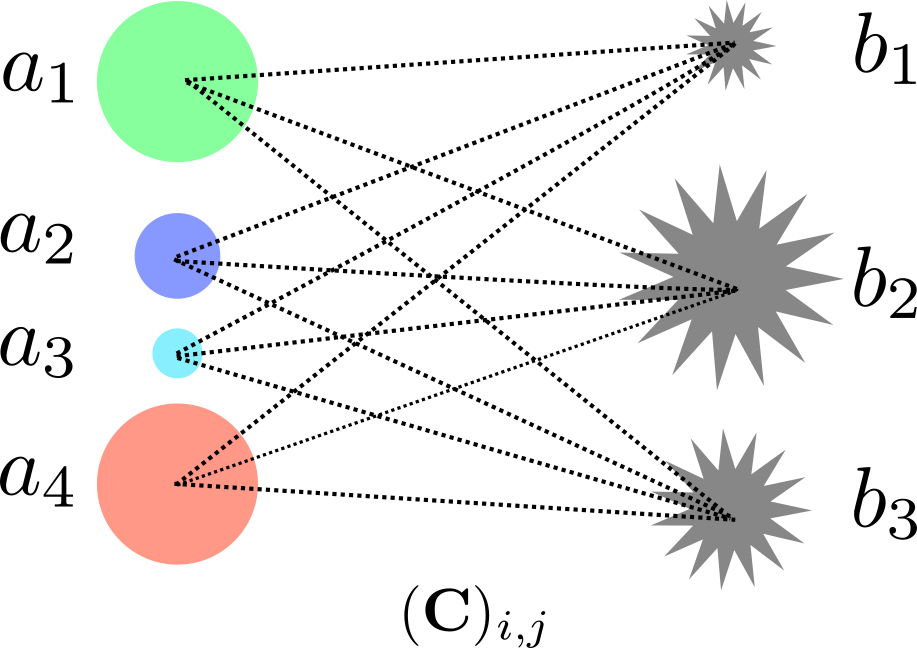
\includegraphics[width=0.95\textwidth]{Network-Flow-Graph}
	\end{subfigure}
	\begin{subfigure}{0.32\textwidth}
		\centering
		\caption{Feasible transportation plan.}
		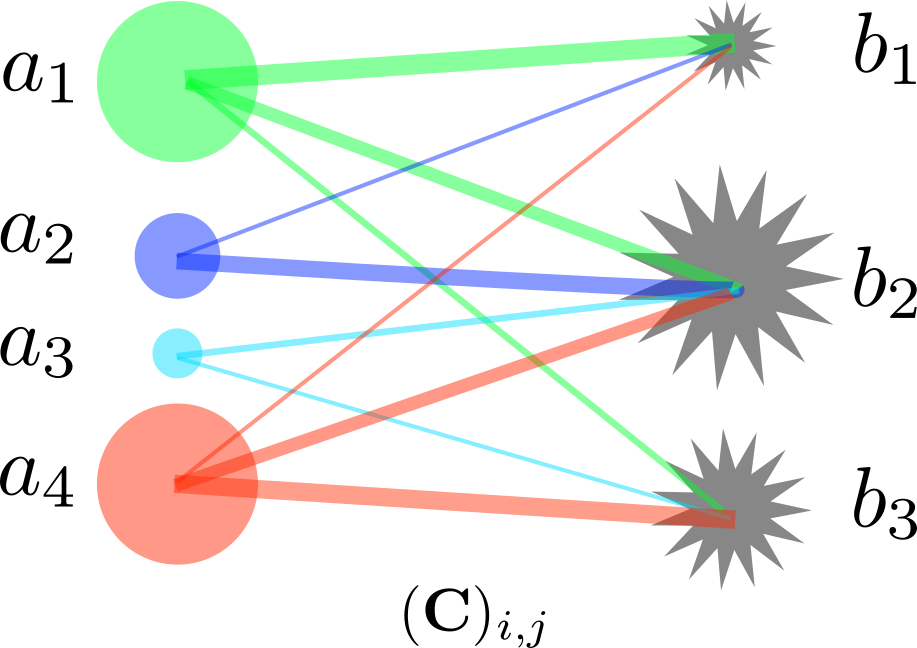
\includegraphics[width=0.95\textwidth]{Network-Feasible-Flow-Graph}
	\end{subfigure}
	\begin{subfigure}{0.32\textwidth}
		\centering
		\caption{Basic Feasible transportation plan.}
		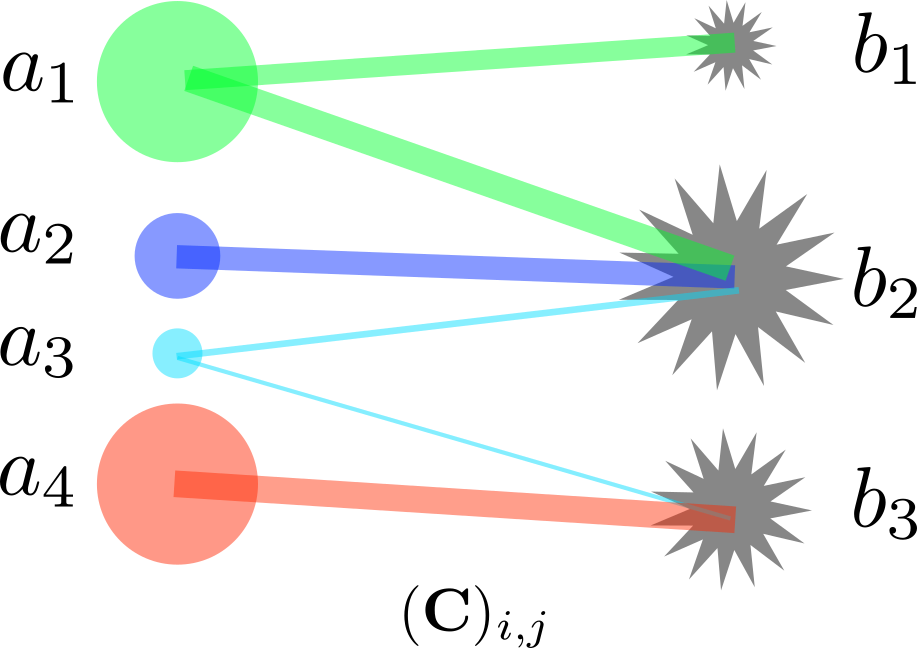
\includegraphics[width=0.95\textwidth]{Network-Basic-Feasible-Flow-Graph}
	\end{subfigure}
 \end{center}
\end{figure}

The network simplex algorithm maintains a basic feasible solution at each stage. Basically, given a basic feasible solution $\pmb{\gamma}$ we compute a complementary pair $(\mathbf{f},\mathbf{g})$ and we check for feasibility. If the complementary pair is not feasible we create a new edge in the graph from one of the pairs $(x_i,y_j)$ violating $\mathbf{C}_{i,j}<(\mathbf{f})_i+(\mathbf{g})_j$ to the edges to the graph. Two situations arise:
\begin{itemize}
	\item The graph keeps its property of being a forest, in this case we only recompute a complementary pair $(\mathbf{f}, \mathbf{g})$ for the new graph. This situation does not represent any change in $\pmb{\gamma}$, it is just the result of the arbitrary way we have found a pair $(\mathbf{f}, \mathbf{g})$.
	\item The graph has a cycle, in this case we need to remove a pair from the graph of $\pmb{\gamma}$, to ensure that we have a forest and modify $\pmb{\gamma}$ in order to be consistent with the new graph. 
	Let $i'_1\to j'_1\to i'_2\to j'_2\to i'_3\to\dots\to i'_K\to j'_K\to i'_1$ the directed path of the cycle we have created. Increase the flow of all the edges $(i', j')$ and decrease it by the same amount in the edges $(j',i')$.
	Let $\tilde{\pmb{\gamma}}$ the new matrix resulting from this operation, that is,
	\begin{equation*}
		\begin{array}{lclc}
		(\tilde{\pmb{\gamma}})_{i'_k,j'_k}&=&({\pmb{\gamma}})_{i'_k,j'_k}+\epsilon&\quad \forall k=1,\dots, K\\
		(\tilde{\pmb{\gamma}})_{i'_{k+1}, j'_k}&=&({\pmb{\gamma}})_{i'_{k+1},j'_{k}}-\epsilon&\quad \forall k=1,\dots,K-1 \\
		(\tilde{\pmb{\gamma}})_{i'_1, j'_k}&=&({\pmb{\gamma}})_{i'_1,j'_{K}}-\epsilon&
		\end{array}
	\end{equation*}
	Take $\epsilon=\min\braces{\gamma_{i_{2}, j_{1}},\dots, \gamma_{i_{K}, j_{K-1}},\gamma_{1,K}}$, in order to keep the constrain $\tilde{\pmb{\gamma}}\geq 0$. Having in this way a tree, since we have removed an edge from a cycle. Finally, we update the transport plan $\pmb{\gamma}\leftarrow\tilde{\pmb{\gamma}}$.
\end{itemize}
Briefly, we initialize the algorithm with a feasible solution $\pmb{\gamma}$ using the North-West rule, resulting into a feasible solution, (not necessarily basic feasible) and we compute a complementary pair $(\mathbf{f},\mathbf{g})$ for $\pmb{\gamma}$. We check for feasibility of the computed pair. If the pair is feasible we have an optimal solution. If the pair $(\mathbf{f},\mathbf{g})$ is not feasible we search for cycles and we make them disappear using the above explained procedure. We compute again the complementary pair $(\mathbf{f}, \mathbf{g}$  and we add to the graph of $\pmb{\gamma}$ the edge corresponding to the indexes that violate the complementary condition, and we continue with the above explained procedure. 

We recommend \cite{Cuturi2018CompOT}, \cite{Orlin1997PolynomialTimeNetworkSimplex} and \cite{Tarjan1997DynamicTreesNetworkSimplex} for a detailed description of the algorithm (for example how to deal with degenerated solutions) and the proofs for the convergence and polynomial order of the Network simplex method.


\section{Sinkhorn-Knopp Algorithm.}
The \emph{Shannon-Neumann anecdote} is a famous conversation between these two great mathematicians Claude Shannon\footnote{Claude Elwood Shannon (April 30, 1916 – February 24, 2001). American mathematician and electrical engineer known as the \textit{Father of the information theory}.} and  John Neumann\footnote{John von Neumann (December 28, 1903 – February 8, 1957). Hungarian-American mathematician and chemical engineering known for applications in many fields covering from computer sciences to physics and mathematics.}, that occurred in the time period fall 1940 to spring 1941 in New Jersey in which von Neumann suggested Shannon to use the term entropy. In April of 1961, Myron Tribus visits Shannon at his office at MIT and questions him about the reason behind his ``entropy'' name adoption.	

Tribus recounts the Shannon interview \cite{Tribus1964Shannon} as such:
\begin{quote}
	I thought of calling it ``information''. But the word was overly used,
	so I decided to call it ``uncertainty''. When I discussed it with John von Neumann, he had a better idea: (...) ``You should call it entropy, for two reasons. In first place your uncertainty has been used in statistical mechanics under that name, so it already has a name. In second place, and more important, no one knows what entropy really is, so in a debate you will always have the advantage.''
\end{quote}


Informally, we can say that the term introduced by Shannon as \textbf{Entropy} quantifies how much information there is in a random signal, language. In relation to our problem, in \cite{Cuturi2018CompOT} is discussed the following: ``In practice actual traffic patterns in a network do not agree with those predicted by the solution of the optimal transport problem. Indeed, the former are more diffuse than the latter, which tend to rely on a few routes as a result of the sparsity of optimal couplings''. \\

The maximum entropy of a set of events is reached when the probability of occurrence is uniform, hence we can interpret the entropy also as a measure of the chaos inside of a system.

In general for any vector representing a probability measure the Shannon's Entropy $H(\mathbf{p}):\Real^{n}\to \Realex$ can be expressed as,
\begin{equation}
H(\mathbf{p})=\begin{cases}
-\infty & \exists i \in \Naturals,\ 1\leq i \leq n \text{ and } \mathbf{p}_{i}=0\\
-\sum_{i=1}^{n}p_i\parentheses{\log(p_i)-1} & \mathbf{p}>0
\end{cases}
\end{equation} 

We can consider $\mathbf{p}=\text{vec}(\pmb{\gamma})$ as the vectorization of a transportation plan matrix. The entropy of the coupling is equivalent to then entropy of its vectorization, that is $H(\pmb{\gamma})=H(\mathbf{p})$. Note that given a matrix with positive entries the Hessian has the form $\delta^2 H(\mathbf{p})= −\diag\parentheses{\frac{1}{\pmb{\gamma}_{i,j}}}$, which implies that is strongly concave in $\mathbf{p}$. \\

The idea is to introduce a strictly convex regularization to the transportation cost in order to have a strictly convex program and hence a unique solution for the problem. 
\begin{equation}
	\Theta(\mu, \nu; \epsilon)=\min_{\pmb{\gamma}\in \Pi(\mu, \nu)}{\anglesbox{\mathbf{C},\pmb{\gamma}}-\epsilon H(\pmb{\gamma})}, \label{eq: Regularized OT}
\end{equation}
where $\epsilon>0$, and $\Pi(\mu,\nu)$ is the set of couplings between two probability measures $
\mu$ and $\nu$ on finite dimensional spaces, identified by vectors $\mathbf{a}$ and $\mathbf{b}$ respectively.

This regularization produces a blurred prediction of the transportation plan given marginals and transportation costs.
\begin{theorem}
	Let $\tilde{\pmb{\gamma}}^{\epsilon}$ the solution for \eqref{eq: Regularized OT} converges to the solution $\pmb{\gamma}^\star$ that has the maximum entropy among the solutions $\pmb{\gamma}$ of the problem \eqref{eq: Optimal Cost Frobenius}  as $\epsilon\rightarrow 0$.
\end{theorem}
\begin{proof}
	Consider a sequence $(\epsilon_\alpha)_{\alpha\in\Naturals} \to 0$ converging to zero, such that $\epsilon_\alpha>0$ for any $\alpha\in\Naturals$. Let $\pmb{\gamma}_\alpha$ the solution of the $\epsilon-$convex program for $\epsilon=\epsilon_\alpha$. The set of couplings $\Pi(\mu,\nu)$ is a closed convex subset of the simplex $\Sigma_{nm}$, therefore we can extract a convergent subsequence (for the sake of simplicity we use the same index of the sequence), such  $\pmb{\gamma}_{\alpha}\rightarrow \pmb{\gamma}^\star$ as $\alpha\rightarrow \infty$.  We are in a closed set therefore $\pmb{\gamma}^\star\in \Pi(\mu,\nu)$. 
	
	In the other hand consider any $\pmb{\gamma}$, such that $\Theta(\mu, \nu)=\anglesbox{\mathbf{C},\pmb{\gamma}}$. Since $\pmb{\gamma}$ is optimal for \eqref{eq: Optimal Cost Frobenius},
	\begin{align}
	0\leq \anglesbox{\mathbf{C},\pmb{\gamma}_\alpha}-\anglesbox{\mathbf{C},\pmb{\gamma}} \label{eq: Optimality Frobenius},
	\end{align}
	and $\pmb{\gamma}_\alpha$ is optimal for $\eqref{eq: Regularized OT}$, we have
	\begin{align}
		0&\leq \parentheses{\anglesbox{\mathbf{C},\pmb{\gamma}}-\epsilon_\alpha H(\pmb{\gamma})}-\parentheses{\anglesbox{\mathbf{C},\pmb{\gamma}_\alpha}-\epsilon_\alpha H(\pmb{\gamma}_\alpha)}\\
		0&\leq \parentheses{\anglesbox{\mathbf{C},\pmb{\gamma}}-\anglesbox{\mathbf{C},\pmb{\gamma}_\alpha}}+\epsilon\parentheses{ H(\pmb{\gamma}_\alpha)- H(\pmb{\gamma})} \label{eq: Optimality Regularized}.
	\end{align}
	Multiplying both sides of the inequality \eqref{eq: Optimality Frobenius} by two and adding it to the inequality \eqref{eq: Optimality Regularized} we have the following inequality,
	\begin{align}
		0\leq \anglesbox{\mathbf{C},\pmb{\gamma}_\alpha}-\anglesbox{\mathbf{C},\pmb{\gamma}}\leq \epsilon\parentheses{H(\pmb{\gamma}_\alpha)-H(\pmb{\gamma})}.
	\end{align}
	We have $H$ and $\anglesbox{\mathbf{C}, \cdot}$ are continuous functions, therefore taking the limit $\alpha\rightarrow \infty$  
	\end{proof}
\subsubsection{Sikhorn Algorithm}
There are many methods that we can use to solve a convex program, for example one of the different versions of the Newton's methods or Backward propagation algorithm. Although recently the so called \textbf{Sinkhorn method} has taken the attention of many researches since it has a high level of parallelism making it GPU\footnote{Graphics Processing Unit.} friendly.
%\section{Applications.}
%\section{Continuous Formulation.}
%\subsection{Beckman Problem and Optimal Transport.}
%\subsection{Proximal Splitting Algorithms.}

\subsection{Examples.}

The following examples were generated using the library of Optimal Transport developed for Python by R\'emi Flamary and Nicolas Courty \cite{flamary2017pot}.

This example takes as cost function $c(x,y)=\frac{1}{2}\abs{x-y}^2$. 